%%%%%%%%%%%%%%%%%%%%%%%%%%%%%%%%%%%%%%%%%%%%%%%%%%%%%%%%%%%%%%%
%
% Welcome to Overleaf --- just edit your LaTeX on the left,
% and we'll compile it for you on the right. If you open the
% 'Share' menu, you can invite other users to edit at the same
% time. See www.overleaf.com/learn for more info. Enjoy!
%
%%%%%%%%%%%%%%%%%%%%%%%%%%%%%%%%%%%%%%%%%%%%%%%%%%%%%%%%%%%%%%%
\documentclass{beamer}
\usepackage[backend=biber,style=numeric, citestyle=ieee]{biblatex}
\addbibresource{bibliography.bib} %Imports bibliography file
\usepackage{svg}
\usepackage{siunitx}
\usepackage{caption}
\captionsetup[figure]{labelformat=empty}
\captionsetup[table]{labelformat=empty}
\usepackage{dcolumn}
\newcolumntype{d}[1]{D{.}{.}{#1}}
\usepackage{booktabs}
\usepackage{hyperref}
\hypersetup{
    colorlinks=true,
    linkcolor=blue,
    filecolor=magenta,      
    urlcolor=cyan
    }
\newcommand{\round}[2]{\num[round-mode=places,round-precision=#1]{#2}}
%Information to be included in the title page:
\title{Stock Market vs. GDP Growth}
\author{Martina Stieger, Flurina Schneider,  \newline Luis Escobar, Till Furger }
\institute{}
\date{\today}

\begin{document}

\frame{\titlepage}


\begin{frame}
\frametitle{Introduction}
\begin{itemize}
\item Examine whether the stock market capitalization grows faster than the 
GDP
\item Focus on United States and compare with Indonesia and Mexico
\item Ratio between a country's market capitalization and its GDP: "Buffet Indicator"; provides insight about under-/overvaluation of stock market 
\item Over the long-term expected to move in sync
\item Several explanations for stock market growing at a faster rate: 
\begin{itemize}
\item Favorable conditions for certain companies
\item Investors optimistic, expect future growth  
\item Stock market overvalued, potential for a bubble
\end{itemize}
\end{itemize}
\end{frame}


\begin{frame}
\frametitle{Introduction}
\begin{itemize}
\item Research gap
\begin{itemize}
\item Current research compares corporate earnings or absolute values of market capitalization
\item Those who do examine growth rates only focus on developed countries or countries of a specific region 
\end{itemize}
\item We compare three different countries across the globe at three different development stages (high income, upper middle and lower middle income)
\end{itemize}
\end{frame}



\begin{frame}
\frametitle{Literature Review}
\begin{itemize}
\item Support of supply-side models: In the long-run, aggregate corporate earnings tend to grow at the same pace as GDP \cite{barra_is_2010}. 
\item Advanced economies: Stock market capitalization and GDP growth in congruence from 1870 to 1980s, ratio tripled after (analysis of 17 advanced economies, 1870-2016). Expansion due to rising equity prices. Profit shift towards listed firms is main driver \cite{kuvshinov_big_2022}. 
\item Relationship between GDP and stock market capitalization for Central and Eastern European countries: "Two-way causality link" between stock market cap and GDP \cite{prats_does_2020}. \item For selected Latin American countries: Economic growth negatively impacted by banking spread, positively impacted by stock market cap  \cite{aali-bujari_impact_2017}. 
\end{itemize}
\end{frame}


\begin{frame}
\frametitle{Methodology}
\begin{itemize}
\item Quantitative part
\begin{itemize}

\item Pull data from Alphavantage, World Bank API, FRED API, Yahoofinance (for years 2000-2022)
\item Provide summary statistics, line plots, box plots, regress SPY on GDP 
\item Develop Rshiny app to compare GDP to the stock market data for the US, Indonesia and Mexico over different time intervals and date ranges
\end{itemize}
\item Qualitative part 
\begin{itemize}
    \item Comparison with selected papers 
\end{itemize}
\end{itemize}
\end{frame}


\begin{frame}
\frametitle{Findings - US}
\begin{itemize}
\item Positive correlation when we regress SPY on US GDP 
\item Average US GDP growth rate lies below the average growth rate of the SPY 
\item Median growth rate of the US GDP lies below the median growth rate of the stock market capitalization 
\item Volatility of SPY growth larger
\end{itemize}
\end{frame}



\begin{frame}
\frametitle{Findings - US}
\begin{figure}[htbp]
	\centering
	\includesvg[width=\textwidth]{figures/histograms_colorblindfriendly}
	\caption{Histograms}
\end{figure}

\end{frame}

\begin{frame}
\frametitle{Findings - US}
\begin{figure}[htbp]
	\centering
	\includesvg[width=\textwidth]{figures/boxplots}
 	\caption{}
\end{figure}

\end{frame}


\begin{frame}
\frametitle{Findings - US}

\begin{table}[H]
	
\begin{tabular}{lrrrr}
\toprule
{} &   US GDP &  SPY 500 &  GDP Growth &  SPY Growth \\
\midrule
count &    82.00 &    82.00 &       81.00 &       81.00 \\
mean  &  4128.13 &   160.36 &        0.01 &        0.03 \\
std   &   452.13 &   101.01 &        0.03 &        0.08 \\
min   &  3263.87 &    55.68 &       -0.06 &       -0.22 \\
25\\%   &  3824.75 &    87.52 &       -0.02 &       -0.00 \\
50\\%   &  4036.64 &   112.79 &        0.02 &        0.04 \\
75\\%   &  4487.54 &   211.11 &        0.03 &        0.07 \\
max   &  5110.95 &   469.53 &        0.08 &        0.20 \\
\bottomrule
\end{tabular}

 	\caption{}
\end{table}

\end{frame}



\begin{frame}
\frametitle{Findings - US}

\begin{figure}[htbp]
	\centering
	\includesvg[width=\textwidth]{figures/regression}
	\caption{}
\end{figure}

\end{frame}

\begin{frame}
\frametitle{Findings - US}

\begin{figure}[htbp]
	\centering
	\includesvg[width=\textwidth]{figures/growth_starting_at_100_colorblindfriendly}
	\caption{}
\end{figure}

\end{frame}

\begin{frame}
\frametitle{Findings - US}

\begin{figure}[htbp]
	\centering
	\includesvg[width=\textwidth]{figures/average_growth_colorblindfriendly}
	\caption{}
\end{figure}

\end{frame}


\begin{frame}
\frametitle{Findings - Global }
\begin{itemize}
\item For considered time period (2000-2022), stock market growth is larger in Indonesia and Mexico compared to the US 
\item Both Indonesia's mean stock index growth rate and GDP growth rate exceed the respective ones of the United States 
\item Mexico's mean GDP growth rate is below the US mean growth GDP rate, while its mean stock index growth rate above the one of the US 
\end{itemize}
\end{frame}

\begin{frame}
\frametitle{Findings - Global}
\begin{itemize}
\item Stock market peaks 
\begin{itemize}
\item 2009 for all 3 countries, highest for Indonesia
\item 2020/07 for all 3 countries, highest for US
\end{itemize}
\item Stock market troughs
\begin{itemize}
\item 2008 for all 3 countries, Indonesia lowest (Financial Crisis)
\item 2020/04 for all 3 countries, Indonesia lowest (Covid)
\end{itemize}


\item GDP peaks
\begin{itemize}
\item 2020/07 for all 3 countries, most extreme for Mexico
\end{itemize}
\item GDP troughs
\begin{itemize}
\item 2020/04 for all 3 countries, most extreme for Mexico (Covid)
\end{itemize}
\end{itemize}
\end{frame}



\begin{frame}
\frametitle{Findings - Global }

\begin{figure}[htbp]
	\centering
	\includesvg[width=\textwidth]{figures/histograms_growth_rates_all}
	\caption{}
\end{figure}

\end{frame}


\begin{frame}
\frametitle{Findings - Global}

\begin{figure}[htbp]
	\centering
	\includesvg[width=\textwidth]{figures/regression_all_incomelevel}
	\caption{}
\end{figure}

\end{frame}

\begin{frame}
\frametitle{Findings - Global}

\begin{figure}[htbp]
	\centering
	\includesvg[width=\textwidth]{figures/growth_lineplots_all}
	\caption{}
\end{figure}

\end{frame}


\begin{frame}
\frametitle{Robustness Checks}
\begin{itemize}
    \item To check the robustness of our findings, we have created an \href{https://flurinaschneider.shinyapps.io/DTFF22/}{interactive app} 
\end{itemize}
\begin{figure}
\centering
\parbox{10cm}{
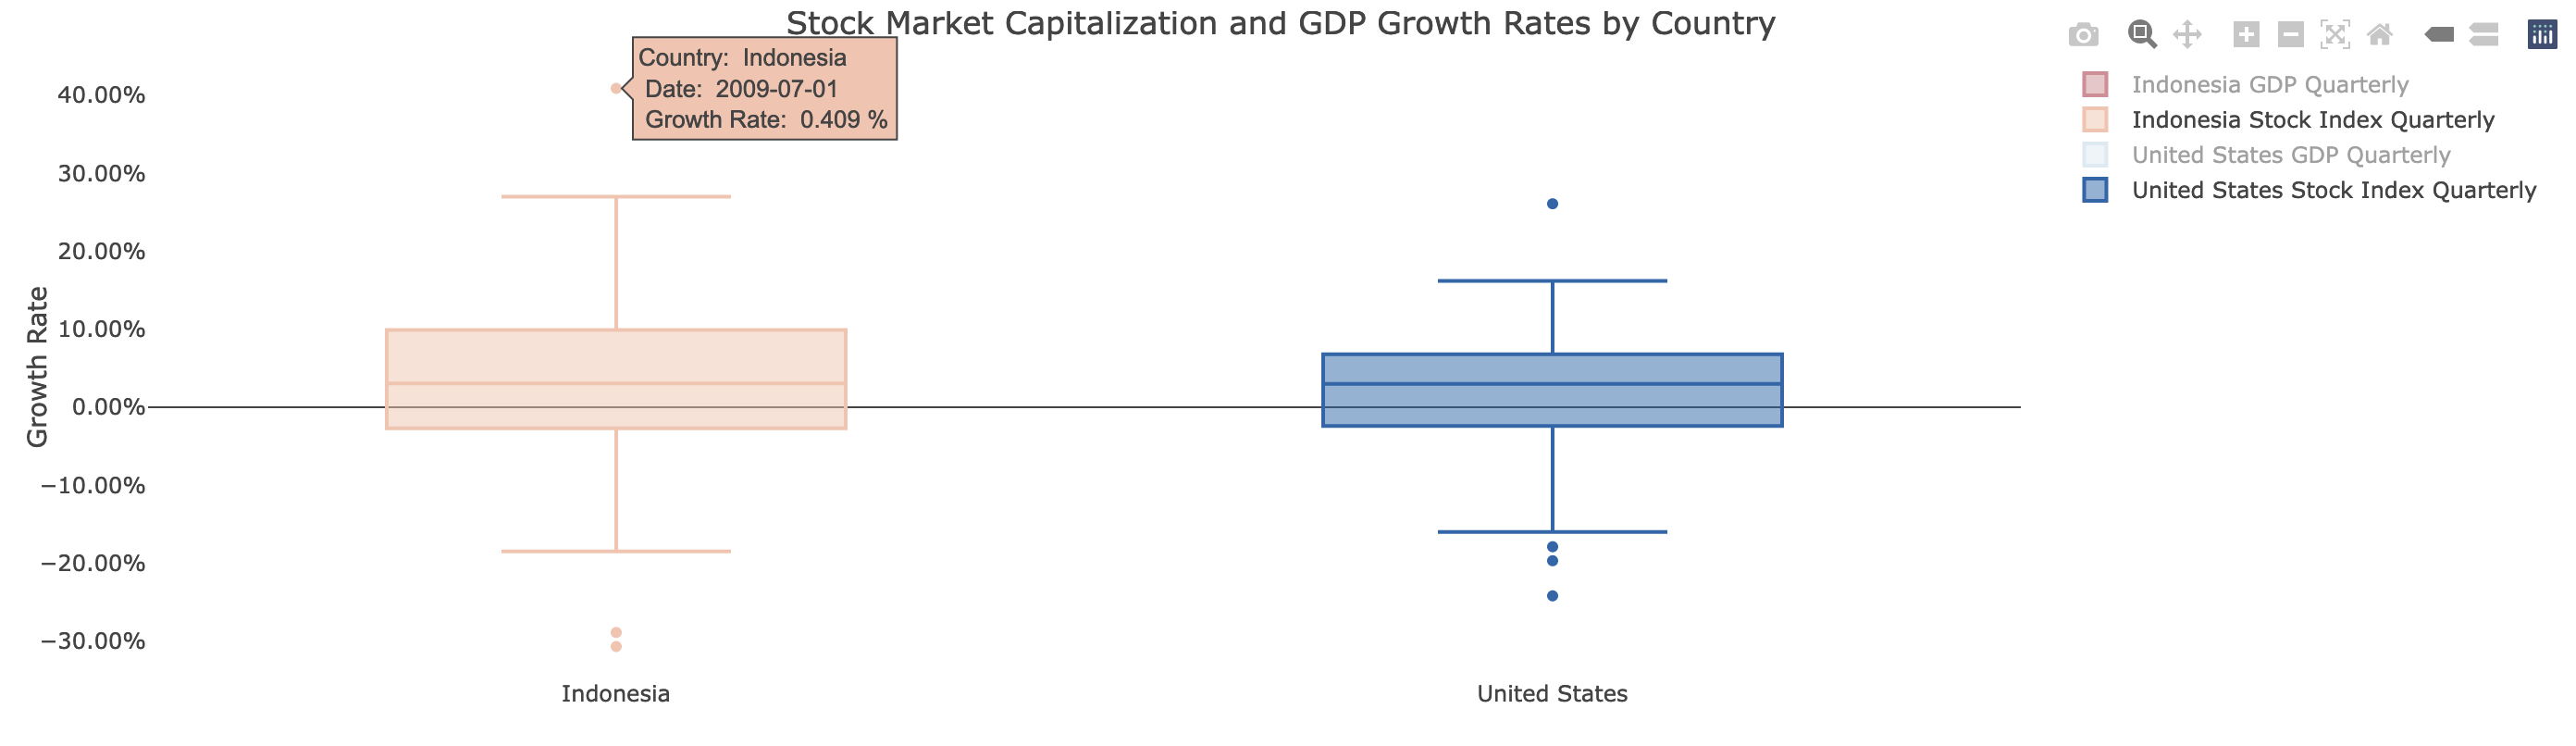
\includegraphics[width=10cm]{reports/figures/robustness_boxplots.png}
\label{fig:2figsA}}
\qquad
\begin{minipage}{10cm}
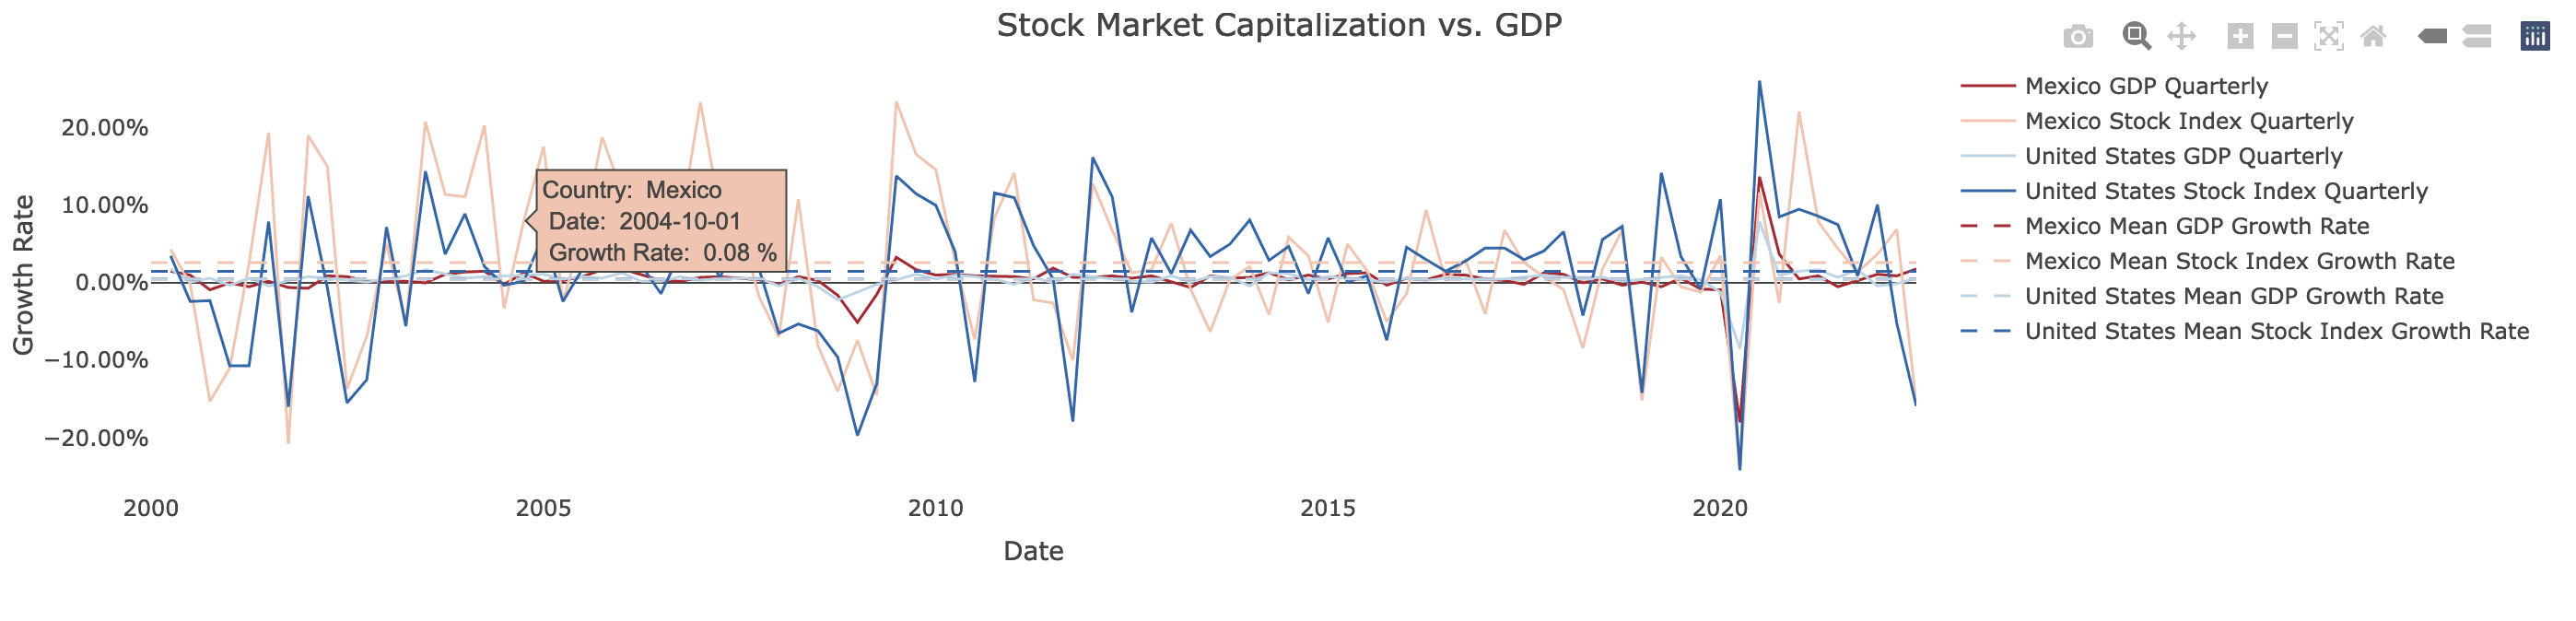
\includegraphics[width=10cm]{reports/figures/robustness_linechart.png}
\label{fig:2figsB}
\end{minipage}
\end{figure}
\end{frame}


\begin{frame}
\frametitle{Results and Discussion}
\begin{itemize}
\item In all examined countries, stock market is growing at a faster rate than GDP
\item The magnitude of the results differ depending on development stage and selected frequency
\item Interpretation according to Buffet Indicator - indication of a potential bubble?
\end{itemize}
\end{frame}


\begin{frame}
\frametitle{Results and Discussion}
\begin{itemize}
\item Limitations 
\begin{itemize}
\item We only look at the aggregate
\item We are not differentiating between industries
\item Take SP500 and SPY as proxy for US (limited selection of companies) 
\item Did not control for region-specific factors  
\end{itemize}
\item Outlook 
\begin{itemize}
\item Increase sample size, include more countries at different development stages to cross-reference
\item Increase time span (provide historical context)
\item Control for additional factors (e.g. region-specific factors)
\end{itemize}
\end{itemize}
\end{frame}



\begin{frame}
\frametitle{Data Sources}
\begin{itemize}
\begin{itemize}

\item For US alone, data for stock market capitalization (using the SPY ETF as a proxy for the S\&P 500) and GDP from \url{https://www.alphavantage.co}. 
    \item Income-level at the country level: \textbf{World Bank API}\footnote{\tiny Documentation: \url{https://datahelpdesk.worldbank.org/knowledgebase/articles/889392-about-the-indicators-api-documentation}}.
    \item GDP quarterly data:  \textbf{FRED API}\footnote{\tiny\url{https://fred.stlouisfed.org/docs/api/fred/}}
    using the \textbf{fredapi} python package\footnote{\tiny https://github.com/mortada/fredapi}.
    \item Stock Indices data: \textbf{Yahoo Finance}\footnote{\tiny \url{https://finance.yahoo.com/}} using the
    \textbf{yfinance} python package\footnote{\tiny \url{https://pypi.org/project/yfinance/}}.
    

 
\end{itemize}
\end{itemize}
\end{frame}


\begin{frame}[allowframebreaks]
\frametitle{References}
\tiny
\printbibliography
\end{frame}


\end{document}
Footer
